\subsection*{Definición de proceso}

Un proceso se define como un conjunto de tareas, actividades o acciones interrelacionadas entre sí que,
a partir de una o varias entradas de información, materiales o de salidas de otros procesos, dan lugar
a una o varias salidas también de materiales (productos) o información con un valor añadido.

Hay tres elementos importantes en un proceso:
\begin{itemize}
	\item Valor agregado: Aquellas que transforman los datos e insumos para crear información y productos o servicios para el cliente.
	\item Traspaso (flujo): Aquellas en las que se entrega de manera interdepartamental o externa la información y productos.
	\item Control: Aquellas que permiten que las actividades de traspaso se lleven a cabo de acuerdo a especificaciones previas de calidad, tiempo y costo establecido.
\end{itemize}
Algunos ejemplos de procesos pueden ser los de producción de bienes, entrega de productos o servicios,
el de gestión de las relaciones con los clientes (habitualmente gestionada por un sistema CRM), el de
desarrollo de la estrategia general de la empresa, el de I+D+I de nuevos productos o servicios, etc.

Estos procesos deben estar correctamente gestionados empleando distintas herramientas de gestión de
procesos (en definitiva gestión de la organización) como puede ser un sistema de planificación de
recursos empresariales (ERP), un sistema de Workflow y otros más.

\subsection*{Procesos de negocio}

Un proceso de negocio es un conjunto de tareas relacionadas lógicamente llevadas a cabo para lograr un
resultado de negocio definido. Cada proceso de negocio tiene sus entradas, funciones y salidas. Las
entradas son requisitos que deben tenerse antes de que una función pueda ser aplicada. Cuando una función
es aplicada a las entradas de un método, tendremos ciertas salidas resultantes.

Es una colección de actividades estructurales relacionadas que producen un valor para la organización,
sus inversores o sus clientes. Es, por ejemplo, el proceso a través del que una organización ofrece sus
servicios a sus clientes.

Un proceso de negocio puede ser parte de un proceso mayor que lo abarque o bien puede incluir otros
procesos de negocio que deban ser incluidos en su función. En este contexto un proceso de negocio
puede ser visto a varios niveles de granularidad. El enlace entre procesos de negocio y generación
de valor lleva a algunos practicantes a ver los procesos de negocio como los flujos de trabajo que
efectúan las tareas de una organización. Los procesos poseen las siguientes características:
\begin{enumerate}
	\item Pueden ser medidos y están orientados al rendimiento
	\item Tienen resultados específicos
	\item Entregan resultados a clientes o “stakeholders”
	\item Responden a alguna acción o evento específico
\end{enumerate}
Los procesos de negocio pueden ser vistos como un recetario para hacer funcionar un negocio y alcanzar
las metas definidas en la estrategia de negocio de la empresa.

Hay tres tipos de procesos de negocio:
\begin{enumerate}
	\item Procesos estratégicos - Estos procesos dan orientación al negocio. Por ejemplo, "Planificar estrategia", "Establecer objetivos y metas".
	\item Procesos centrales – Estos procesos dan el valor al cliente, son la parte principal del negocio. Por ejemplo, “Repartir mercancías”
	\item Procesos de soporte – Estos procesos dan soporte a los procesos centrales. Por ejemplo, “contabilidad”, “Servicio técnico”.
\end{enumerate}
Los procesos de negocio consisten en subprocesos, decisiones y actividades.

Un subproceso es parte un proceso de mayor nivel que tiene su propia meta, propietario, entradas y salidas.

Las actividades son partes de los procesos de negocio que no incluyen ninguna toma de decisión ni vale
la pena descomponer (aunque ello sea posible). Por ejemplo, “Responde al teléfono”, “Haz una factura”.

Un proceso de negocio es usualmente el resultado de una Reingeniería de Procesos. El modelado de procesos
es usado para capturar, documentar y rediseñar procesos de negocio.

Vamos a decir que en la época de Taylor un operario realizaba una tarea especifica, y luego se cambió esa
perspectiva en torno a los procesos que son realizados por un trabajo en equipo teniendo en cuenta al cliente
el cual fija las ritmos de los resultados.

Esto facilita el acercamiento y el acuerdo con los clientes, mejora la motivación de los empleados y existe
una mayor facilidad para responder a cambios en el contexto.

Para aplicar los procesos se deben tener claras las tareas, una estructura jerárquica y una tendencia a la
interacción y comunicación vertical.

\subsection*{Metodología esquemática de Reingeniería de Procesos}

Como extremo ideal, se puede establecer una metodología de "papel en blanco", en la que se reinventa toda la
estructura y funcionamiento del proceso o de la organización. Se mantienen los objetivos y estrategias básicas
del negocio, pero se adopta una libertad total de ideas. Esta metodología se puede restringir aprovechando en
mayor o menor medida los procesos ya existentes, haciéndose así un rediseño parcial del proceso.

En cualquiera de los casos, la reingeniería de procesos crea cambios directos y radicales que requieren unas
circunstancias en la organización para adoptarse con éxito:
\begin{itemize}
	\item Sensibilización al cambio.
	\item Planeación estratégica.
	\item Automatización.
	\item Gestión de Calidad Total.
	\item Reestructuración Organizacional.
	\item Mejora Continua.
	\item Valores compartidos.
	\item Perspectiva individual.
	\item Comportamiento en el lugar de trabajo.
	\item Resultados finales.
\end{itemize}
Las etapas de la reingeniería pueden ser las siguientes:
\begin{itemize}
	\item Identificación de los procesos estratégicos y operativos existentes o necesarios, y creación de un mapa (un modelo) de dichos procesos.
	\item Jerarquización del mapa de procesos para su rediseño, y determinación de los procesos clave, aquellos que se abordarán primero o con mayor interés.
	\item Desarrollo de la visión de los nuevos procesos mejorados.
	\item Reingeniería (creación y rediseño) de procesos, realizada por consultores externos, especialistas internos, o una mezcla de ambos.
	\item Preparación y prueba de los nuevos procesos (procesos pilotos).
	\item Procesos posteriores de mejora continúa.
\end{itemize}

\subsection*{La cadena de Valor}

La cadena de valor fue descrita y popularizada por Michael E. Porter en su best-seller de 1985: Competitive Advantage: Creating and Sustaining Superior Performance. New York, NY The Free Press.
Algunas ideas importantes sobre la Cadena de Valor:
\begin{itemize}
	\item Disgrega actividades importantes de la empresa.
	\item La cadena de valor comprende desde el proveedor hasta el cliente.
	\item El obtener y mantener ventajas competitivas depende de comprender y manejar la cadena de valor.
	\item La cadena de valor en las empresas difiere de la empresa, el sector, historia, su estrategia, etc.
\end{itemize}
Tenemos que tener claro que cada empresa es un conjunto de actividades que lleva a cabo para:
\begin{itemize}
	\item Diseñar
	\item Producir
	\item Llevar al mercado
	\item Entregar
	\item Apoyar sus productos
\end{itemize}

Cada actividad de valor emplea insumos, recursos humanos, algún tipo de tecnología para desempeñar su función.
Cada actividad de valor utiliza y crea información. (por ejemplo: datos del comprador, parámetros de desempeño de maquinaria, estadísticas de fallas del producto, etc.).

La Cadena de Valor categoriza las actividades que producen valor añadido en una organización. Se dividen en dos tipos de actividades:
\begin{itemize}
	\item Las actividades primarias que conforman la creación física del producto, las actividades relacionadas con su venta y la asistencia post-venta. Se dividen en:
	\begin{itemize}
		\item Logística interna: recepción, almacenamiento y distribución de las materias primas.
		\item Operaciones (producción): recepción de las materias primas para transformarlas en el producto final.
		\item Logística externa: almacenamiento de los productos terminados y distribución del producto al consumidor.
		\item Ventas y Marketing: actividades con las cuales se da a conocer el producto.
		\item Servicios post-venta (mantenimiento): actividades destinadas a mantener o realizar el valor del producto. Ej: garantías
	\end{itemize}
	\item Estas actividades son apoyadas por las también denominadas actividades secundarias:
	\begin{itemize}
		\item Infraestructura de la organización: actividades que prestan apoyo a toda la empresa, como la planificación, contabilidad, finanzas...
		\item Dirección de recursos humanos: búsqueda, contratación y motivación del personal.
		\item Desarrollo de tecnología (investigación y desarrollo): obtención, mejora y gestión de la tecnología.
		\item Abastecimiento (compras): proceso de compra de los materiales.
	\end{itemize}
\begin{center}
	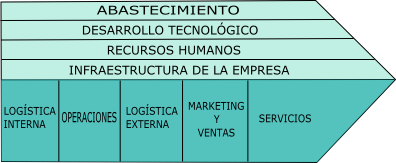
\includegraphics[height=4cm]{images/cadenaDeValor}
\end{center}

\end{itemize}

\subsubsection*{Tipos de Actividad}
Dentro de cada categoría de actividades primarias y de apoyo, hay tres tipos de actividades que juegan un papel diferente en la ventaja competitiva:
\begin{itemize}
	\item Directas: Actividades implicadas directamente en la creación de valor para el comprador: ensamble, maquinado de partes, operación de la fuerza de ventas,etc.
	\item Indirectas: Actividades que hacen posible el desempeñar las actividades directas en una base continua, como mantenimiento, programación, operación de las instalaciones, etc.
	\item Seguro de calidad: Actividades que aseguran la calidad de otras actividades (monitoreo, inspección, pruebas, revisión, etc.)
\end{itemize}
Ademas Para cada actividad de valor añadido han de ser identificados los generadores de costes y valor.

\subsubsection*{El marco de la cadena}

La cadena de valor enseguida se puso en el frente del pensamiento de gestión de empresa como una poderosa
herramienta de análisis para planificación estratégica. Su objetivo último es maximizar la creación de valor
mientras se minimizan los costos. De lo que se trata es de crear valor para el cliente, lo que se traduce
en un margen entre lo que se acepta pagar y los costos incurridos.

La cadena de valor ayuda a determinar las actividades que permiten generar una Ventaja Competitiva (también
expresado por Michael Porter). Tener una ventaja competitiva es tener una rentabilidad relativa superior a
los rivales en el sector industrial en el cual se compite, la cual tiene que ser sustentable en el tiempo.
Rentabilidad significa un margen entre los ingresos y los costos. Cada actividad que realiza la empresa debe
generar el mayor posible. De no ser así, debe costar lo menos posible, con el fin de obtener un margen superior
al de los rivales. Las Actividades de la cadena de valor son múltiples y además complementarias (relacionadas).
El conjunto de actividades de valor que decide realizar una unidad de negocio es a lo que se le llama estrategia
competitiva (también expresado por Porter) o estrategia del negocio (diferente a las estrategias corporativas
o a las estrategias de un área funcional).

El concepto ha sido extendido más allá de las organizaciones individuales. También puede ser aplicado a cadenas
de suministro completas así como a redes de distribución. La puesta a disposición de un conjunto de productos y
servicios al consumidor final moviliza diferentes actores económicos, cada uno de los cuales gestiona su cadena
de valor. Las interacciones sincronizadas de esas cadenas de valor locales crean una cadena de valor ampliada que
puede llegar a ser global. Capturar el valor generado a lo largo de la cadena es la nueva aproximación que han
adoptado muchos estrategas de la gestión. A base de explotar la información que se dirige hacia arriba y hacia
abajo dentro de la cadena, las compañías pueden intentar superar los intermediarios creando nuevos modelos de negocio.

\subsubsection*{Valor Agregado vs Cadena de Valor}
Valor agregado es el precio de venta menos el costo de la materia prima comprada.
El valor agregado no es una base sólida de análisis de costos y ventajas competitivas ya que no distingue el costo de materias primas.
De muchos otros insumos que son adquiridos (comprados) que se utilizan en las actividades de una empresa.
El comportamiento de los costos no puede ser comprendido sin examinar simultáneamente los costos de los insumos usados para lograrlos.
En la Cadena de Valor realza las relaciones entre la empresa y sus proveedores, lo que puede reducir el costo o aumentar la diferenciación.
(la diferencia que una empresa establece al proporcionar algo único que es valioso para los compradores más allá de ofrecer un precio bajo).

\subsubsection*{Eslabones dentro de la Cadena de Valor}
La Cadena de Valor es un sistema de actividades interdependientes relacionadas por eslabones o relaciones entre la manera en que se desempeñe una actividad y el costo o desempeño de otra.
Los eslabones pueden llevar a la ventaja competitiva de dos maneras:
\begin{itemize}
	\item Optimización
	\item Coordinación
\end{itemize}
Los eslabones surgen de:
\begin{itemize}
	\item La misma función puede ser desempeñada de diferentes formas.
	\item El costo de desempeño de las actividades directas se puede mejorar por mayores esfuerzos de actividades indirectas.
	\item Actividades desempeñadas dentro de una empresa reducen la necesidad de mostrar, explicar o dar servicio a un producto en el campo.
	\item Las funciones de seguro de calidad pueden ser desempeñadas de diferentes maneras.
\end{itemize}
Los eslabones son cruciales en la Cadena de Valor pero muchas veces son sutiles y pasan desapercibidos.
La identificación de los eslabones es un proceso de búsqueda de maneras en que las que cada actividad de valor afecta o es afectada por otras.

\subsubsection*{Eslabones Verticales}
Los eslabones no sólo existen dentro de la Cadena de Valor de la empresa, sino entre la cadena de una empresa y las Cadenad de Valor de los proveedores y los canales.
También hay cadena de valor de comprador y la forma en que se relaciona con la Cadena de Valor de la empresa, marca diferenciación.

La Cadena de Valor despliega el valor total y consiste de las actividades de valor y del margen.
El margen es la diferencia entre el valor total y el costo colectivo de desempeñar las actividades de valor.

\newpage
